% !TeX spellcheck = de_CH
% /*
%  * ----------------------------------------------------------------------------
%  * "THE BEER-WARE LICENSE" (Revision 42):
%  * <michi.wieland@hotmail.com> wrote this file. As long as you retain this notice you
%%  * can do whatever you want with this stuff. If we meet some day, and you think
%  * this stuff is worth it, you can buy me a beer in return. Michael Wieland
%  * ----------------------------------------------------------------------------
%  */

\documentclass[
a4paper,
oneside,
10pt,
fleqn,
headsepline,
toc=listofnumbered, 
bibliography=totocnumbered]{scrartcl}

% deutsche Trennmuster etc.
\usepackage[T1]{fontenc}
\usepackage[utf8]{inputenc}
\usepackage[english, ngerman]{babel} % \selectlanguage{english} if  needed
\usepackage{lmodern} % use modern latin fonts

% Custom commands
\newcommand{\AUTHOR}{Michael Wieland}
\newcommand{\INSTITUTE}{Hochschule für Technik Rapperswil}
\newcommand{\GITHUB}{https://github.com/michiwieland/hsr-zusammenfassungen}
\newcommand{\LICENSEURL}{https://en.wikipedia.org/wiki/Beerware}
\newcommand{\LICENSE}{
"THE BEER-WARE LICENSE" (Revision 42):
<michi.wieland@hotmail.com> wrote this file. As long as you retain this notice you
can do whatever you want with this stuff. If we meet some day, and you think
this stuff is worth it, you can buy me a beer in return. Michael Wieland	
}

% Jede Überschrift 1 auf neuer Seite
\let\stdsection\section
\renewcommand\section{\clearpage\stdsection}

% Multiple Authors
\usepackage{authblk}

% Include external pdf
\usepackage{pdfpages}

% Layout / Seitenränder
\usepackage{geometry}

% Inhaltsverzeichnis
\usepackage{makeidx} 
\makeindex

\usepackage{url}
\usepackage[pdfborder={0 0 0}]{hyperref}
\usepackage[all]{hypcap}
\usepackage{hyperxmp} % for license metadata

% Glossar und Abkürzungsverzeichnis
\usepackage[acronym,toc,nopostdot]{glossaries}
\glossarystyle{altlist}
\usepackage{xparse}
\DeclareDocumentCommand{\newdualentry}{ O{} O{} m m m m } {
	\newglossaryentry{gls-#3}{
		name={#4 : #5},
		text={#5\glsadd{#3}},
		description={#6},
		#1
	}
	\makeglossaries
	\newacronym[see={[Siehe:]{gls-#3}},#2]{#3}{#4}{#5\glsadd{gls-#3}}
}
\makeglossaries

% Mathematik
\usepackage{amsmath}
\usepackage{amssymb}
\usepackage{amsfonts}
\usepackage{enumitem}

% Images
\usepackage{graphicx}
\graphicspath{{images/}} % default paths

% Boxes
\usepackage{fancybox}

%Tables
\usepackage{tabu}
\usepackage{booktabs} % toprule, midrule, bottomrule
\usepackage{array} % for matrix tables

% Multi Columns
\usepackage{multicol}

% Header and footer
\usepackage{scrlayer-scrpage}
\setkomafont{pagehead}{\normalfont}
\setkomafont{pagefoot}{\normalfont}
\automark*{section}
\clearpairofpagestyles
\ihead{\headmark}
\ohead{\AUTHOR}
\cfoot{\pagemark}

% Pseudocode
\usepackage{algorithmic}
\usepackage[linesnumbered,ruled]{algorithm2e}

% Code Listings
\usepackage{listings}
\usepackage{color}
\usepackage{beramono}

\definecolor{bluekeywords}{rgb}{0,0,1}
\definecolor{greencomments}{rgb}{0,0.5,0}
\definecolor{redstrings}{rgb}{0.64,0.08,0.08}
\definecolor{xmlcomments}{rgb}{0.5,0.5,0.5}
\definecolor{types}{rgb}{0.17,0.57,0.68}

\lstdefinestyle{visual-studio-style}{
	language=[Sharp]C,
	columns=flexible,
	showstringspaces=false,
	basicstyle=\footnotesize\ttfamily, 
	commentstyle=\color{greencomments},
	morekeywords={partial, var, value, get, set},
	keywordstyle=\bfseries\color{bluekeywords},
	stringstyle=\color{redstrings},
	breaklines=true,
	breakatwhitespace=true,
	tabsize=4,
	numbers=left,
	numberstyle=\tiny\color{black},
	frame=lines,
	showspaces=false,
	showtabs=false,
	escapeinside={£}{£},
}

\definecolor{DarkPurple}{rgb}{0.4, 0.1, 0.4}
\definecolor{DarkCyan}{rgb}{0.0, 0.5, 0.4}
\definecolor{LightLime}{rgb}{0.3, 0.5, 0.4}
\definecolor{Blue}{rgb}{0.0, 0.0, 1.0}

\lstdefinestyle{cevelop-style}{
	language=C++,  
	columns=flexible,
	showstringspaces=false,     
	basicstyle=\footnotesize\ttfamily, 
	keywordstyle=\bfseries\color{DarkPurple},
	commentstyle=\color{LightLime},
	stringstyle=\color{Blue}, 
	escapeinside={£}{£}, % latex scope within code      
	breaklines=true,
	breakatwhitespace=true,
	showspaces=false,
	showtabs=false,
	tabsize=4,
	morekeywords={include,ifndef,define},
	numbers=left,
	numberstyle=\tiny\color{black},
	frame=lines,
}

\lstdefinestyle{eclipse-style}{
	language=Java,  
	columns=flexible,
	showstringspaces=false,     
	basicstyle=\footnotesize\ttfamily, 
	keywordstyle=\bfseries\color{DarkPurple},
	commentstyle=\color{LightLime},
	stringstyle=\color{Blue}, 
	escapeinside={£}{£}, % latex scope within code      
	breaklines=true,
	breakatwhitespace=true,
	showspaces=false,
	showtabs=false,
	tabsize=4,
	morekeywords={length},
	numbers=left,
	numberstyle=\tiny\color{black},
	frame=lines,
}
\lstset{style=eclipse-style}



% Theorems \begin{mytheo}{title}{label}
\usepackage{tcolorbox}
\tcbuselibrary{theorems}
\newtcbtheorem[number within=section]{definiton}{Definition}%
{fonttitle=\bfseries}{def}
\newtcbtheorem[number within=section]{remember}{Merke}%
{fonttitle=\bfseries}{rem}
\newtcbtheorem[number within=section]{hint}{Hinweis}%
{fonttitle=\bfseries}{hnt}

% Dokumentinformationen
\newcommand{\SUBJECT}{Zusammenfassung}
\newcommand{\TITLE}{Verteilte Software Systeme}

\loadglsentries{glossar}

% pdf metadata
\hypersetup{
	pdfauthor={\AUTHOR},
	pdftitle={\SUBJECT \TITLE},
	pdfcopyright={\LICENSE},
	pdflicenseurl={\LICENSEURL}
}

\begin{document}
	
% Front page
\title{\TITLE}
\subject{\SUBJECT}
\author{\AUTHOR}
\affil{\INSTITUTE}
\date{\today}
\maketitle

\vfill

% Participate
\paragraph{Mitmachen} \hfill \\
Falls Du an diesem Dokument mitarbeiten willst, kannst Du das Dokument
auf GitHub unter \url{\GITHUB} forken.

% Licence
\paragraph{Lizenz} \hfill \\
\LICENSE

% Table of contents
\tableofcontents


% Glossar and acronyms (if included \loadglsentries{glossar})
\printglossary[type=\acronymtype]
\printglossary
\glsaddall


\section{Introduction}

Distributes System: A distributed system is a collection of independent computers that appears to its users as a single coherent system.


\subsection{Herausforderungen und Ziele VSS}
Herausforderungen:
\begin{itemize}
	\item Komplexe Kommunikation / Systeme
	\item Performanzprobleme
	\item Zuverlässigkeit
	\item Transaktionssicherheit
\end{itemize}
Ziele:
\begin{itemize}
	\item Remote-Kommunikation heterogener Anwendungsteile (Interoperabilität)
	\item Hohe Benutzerzahlen (Scalability)
	\item Fault Tolerance (Robustness)
\end{itemize}

\subsubsection{Häufige Fehlannahmen}
Eight Fallacies of Distributed Systems (dt. Trugschlüsse, nicht zutreffende Annahmen, siehe http://www.rgoarchitects.com/Files/fallacies.pdf):
\begin{itemize}
	\item The network is reliable.
	\item Latency is zero.
	\item Bandwidth is infinite.
	\item The network is secure.
	\item Topology doesn't change.
	\item There is one administrator.
	\item Transport cost is zero.
	\item The network is homogeneous.
\end{itemize}

Fowler’s First Law of Distributed Object Design, siehe: http://www.drdobbs.com/errant-architectures/184414966
\begin{itemize}
	\item Don’t distribute your objects! 
\end{itemize}

\subsubsection{ACID}
ACID ist eine Voraussetzung für die Verlässlichkeit von verteilten Systemen.
\begin{description}
	\item[Atomicity] Ganz oder gar nicht
	\item[Consistency] Nach jeder Transaktion müssen die Daten konsistent sein
	\item[Isolation] Nebenläufige Ausführungen beeinflussen sich nicht
	\item[Durability] Änderungen an den Daten bleiben persistent
\end{description}

\subsection{Middlewares}

Üblicherweise wird ein verteiltes Software System über eine Middleware gesteuert. Gründe für die Einführung von Middleware:
\begin{itemize}
	\item Überwindung von Heterogenität (Interoperabilität, Transparenz)
	\item Vereinfachte Erstellung verteilter Anwendungen (Produktivität)
\end{itemize}

Die Middleware kann folgende Funktionen umfassen: Kommunikation, Naming, Events, Security, Transactions etc.

\subsubsection{Arten von Middlewares}

\begin{description}
	\item[Kommunkationsorienterte Middleware] Abstraktion Netzwerkzugriff. Implementierungen: z.B. Sockets (low-level Protokolle)
	\item[Anwendungsorientierte Middleware] Weitreichente Unterstützung verteilter Anwendung z.B. Discovery, Sicherheit, Zuverlässigkeit, verteilte Transaktionen, Sessions. Implementierungen: CORBA IDL, RMI interfaces, WSDL/SOAP Web Services (high-level Protokolle)
\end{description}

\subsection{Architekturstile}

\begin{figure}[h]
	\centering
	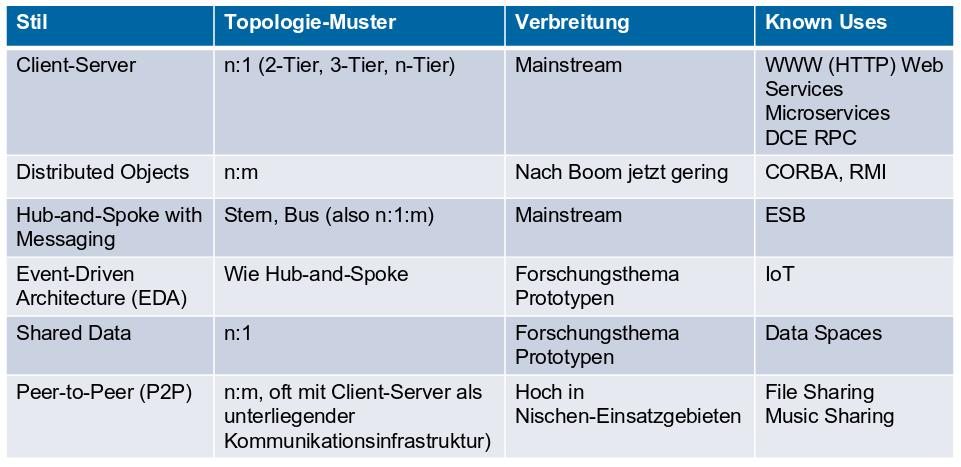
\includegraphics[width=0.7\linewidth]{img/vss_architecture}
	\caption{Architekturen von VSS}
	\label{fig:vssarchitecture}
\end{figure}

\subsubsection{Design Aspects}
\begin{itemize}
	\item Communication Topology (Clients, Network, Server Nodes)
		\begin{itemize}
			\item One client, one server? Many clients for one server? Dynamic setup?
		\end{itemize}
	\item Location Autonomy (Transparency)
		\begin{itemize}
			\item Real address vs. virtual address (what if a server is moved?)
		\end{itemize}
	\item Invocation and Message Semantics
		\begin{itemize}
			\item Bytestream vs. Document vs. Procedure vs. Remote Object
		\end{itemize}
	\item Timeout Management
		\begin{itemize}
			\item 1ms? 30 seconds? Infinite?
		\end{itemize}
	\item Error Handling
		\begin{itemize}
			\item Retry request? 
			\item Make server idempotent?
		\end{itemize}
\end{itemize}

\subsection{Tiers}

\begin{itemize}
	\item Two-Tier (Aufteilung in Client und Server)
	\item Three-Tier (Aufteilung in Clients, Logic und Backend bzw. oft Client, Applikation und Datenbank)
\end{itemize}

\subsection{Integrationen}

\begin{itemize}
\item File Transfer
\item shared Database (Common)
\item Remote Procedure Invocation
\item Messaging (Common exchange): Üblicherweise identifikation der Response über request ID
\end{itemize}

\subsection{Transparency}

\begin{figure}[h]
	\centering
	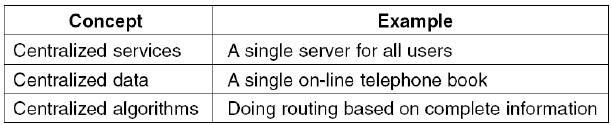
\includegraphics[width=0.7\linewidth]{img/centralized_concept_services}
	\caption{Scalability Issues / Centralized Concept Services}
	\label{fig:centralizedconceptservices}
\end{figure}


\begin{figure}[h]
	\centering
	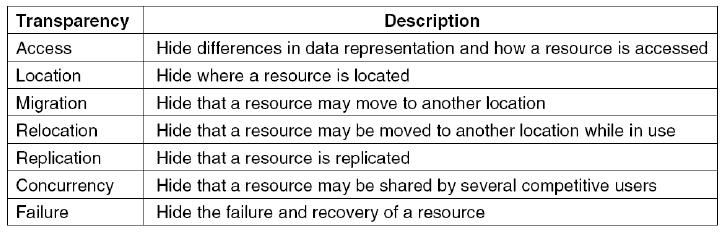
\includegraphics[width=0.7\linewidth]{img/transparency_types}
	\caption{Transparancy Types ISO 1995}
	\label{fig:transparencytypes}
\end{figure}


\subsection{Dimensionen der Schwierigkeit}

\begin{description}
	\item[Nebenläufigkeit] gleichzeitig / concurrency
	\item[Persistenz/Transparenz] Sichbarkeit der Verteilung / tatsächlichen Orten
	\item[Verteilung/Transparenz] Sichbarkeit, ob eine Ressource Lokal/Verteilt ist
\end{description}

\subsection{Inter Process Communication (IPC)}
Die drei Varianten unterscheiden sich in Punkto Unterstützung von Sicherheit, Zuverlässigkeit, Transaktionsmanagement, Kopplung und QoS.
\begin{figure}[h]
	\centering
	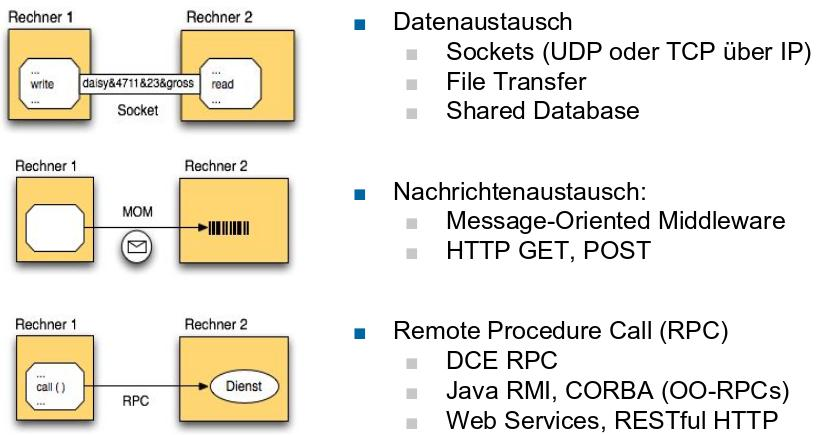
\includegraphics[width=0.7\linewidth]{img/ipc_abstraction_layers}
	\caption{IPC Abstraktionsebenen}
	\label{fig:ipcabstractionlayers}
\end{figure}


\section{Technologien}
\subsection{Sockets}

Basis Mechanismus für alle komplexere Verfahren (HTTP, RMI, etc.)
\begin{itemize}
	\item Austausch von Byteströmen
	\item Socket ist Verbindung zwischen zwei Kommunikationsendpunkten (IP/Port)
	\item Zwei Rollen: Client/Server
\end{itemize}

Vorteile:
\begin{itemize}
	\item Flexibel und mächtig
	\item Effizient (hinsichtlich Network Traffic)
	\item Genügt z.B. um aktualisierte Informationen zu übermitteln
\end{itemize}

Nachteile:
\begin{itemize}
	\item Nur übermitteln von Rohdaten
	\item Eigenes Konstruieren und Parsen von Byteströmen
	\item Message Exchange Pattern (MEP) muss selbst spezifiziert, implementiert und überprüft werden. Das MEP definiert die Reihenfolge der \lstinline|send()| und \lstinline|receive()| Calls zwischen Client/Server.
	\item Client \& Server müssen State-Informationen vorhalten.
\end{itemize}

\clearpage

\subsubsection{TCP}
\begin{figure}[h!]
	\centering
	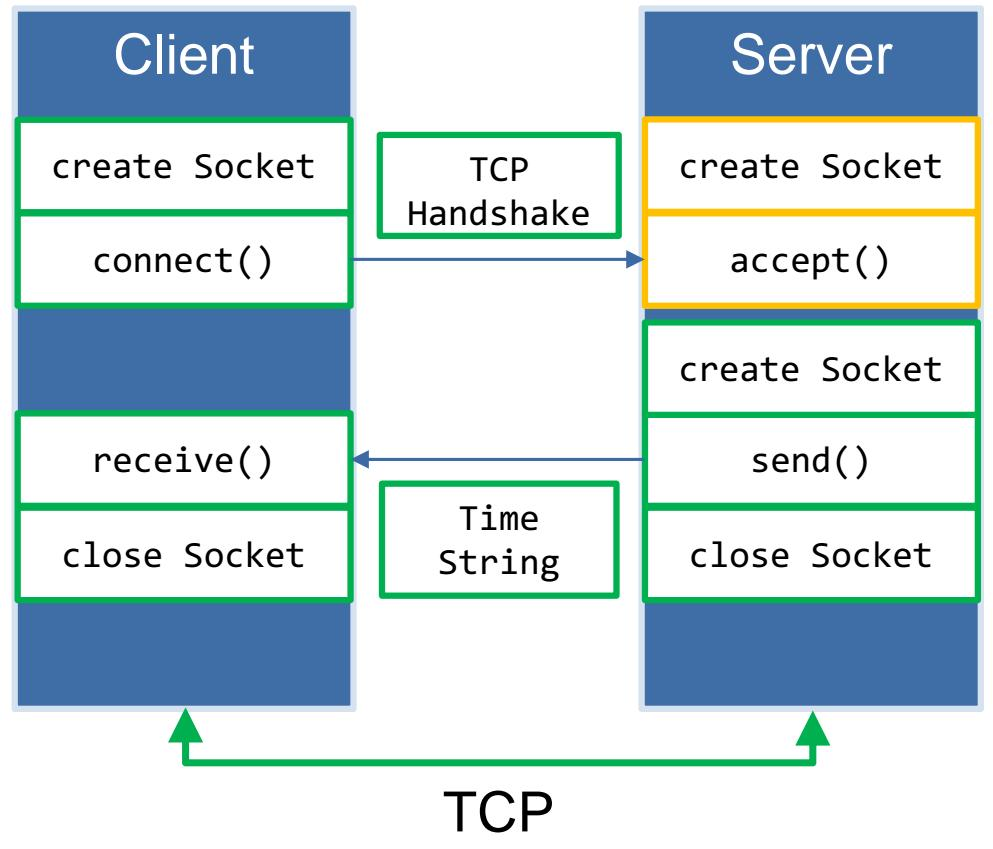
\includegraphics[width=0.5\linewidth]{img/tcp_socket}
	\caption{TCP Socket}
	\label{fig:tcpsocket}
\end{figure}

\paragraph{Client}
\begin{enumerate}
	\item Find the IP address and port number of the server
	\item Create a TCP Socket
	\item Connect the Socket to the server (server must be up and listening for new requests)
	\item Send data to / receive data from server using the socket
	\item Close the connection
\end{enumerate}

\begin{lstlisting}
public class DaytimeTCPClient {
	
	private final String host = "localhost";
	private final int port = 5000;
	
	private void connectToServer() throws Exception {
		try (Socket server = new Socket(host, port)) {
			BufferedReader in = new BufferedReader(new InputStreamReader(server.getInputStream()));
			String date = in.readLine();
			System.out.println(date);
		}
		
	}
	
	public static final void main(String[] args) throws Exception {
		DaytimeTCPClient client = new DaytimeTCPClient();
		client.connectToServer();
	}
}
\end{lstlisting}

\paragraph{Server}
\begin{enumerate}
	\item Find the IP address and port number of the server
	\item Create a TCP server socket
	\item Bind server socket to server IP and port number (this is the port to which clients will 
	connect)
	\item Accept new connection from client (returns client Socket that represents the client 
	which is connected)
	\item Send data to / receive data from client, using client socket
	\item Close the connection with client  
\end{enumerate}

\begin{lstlisting}
public class DaytimeTCPServer {
	
	private final int port = 5000;
	
	private void listen() throws Exception {
		try (ServerSocket server = new ServerSocket(port)) {
			while (true) {
				Socket client = server.accept();
				
				PrintWriter out = new PrintWriter(client.getOutputStream(), true);
				Date date = new Date();
				out.println(date);
			}
		}
	}
	
	public static void main(String[] args) throws Exception {
		DaytimeTCPServer server = new DaytimeTCPServer();
		server.listen();
	}
}
\end{lstlisting}

\clearpage

\subsubsection{UDP}
Wird eingesetzt für Low-Latency, State-less Übertragungen, bei denen Paketverlust keine (schlimme Konsequenzen hat). Es gibt keine Garantie für die Datenübertragung, Reihenfolge und Atomizität der Pakete.
\begin{figure}[h!]
	\centering
	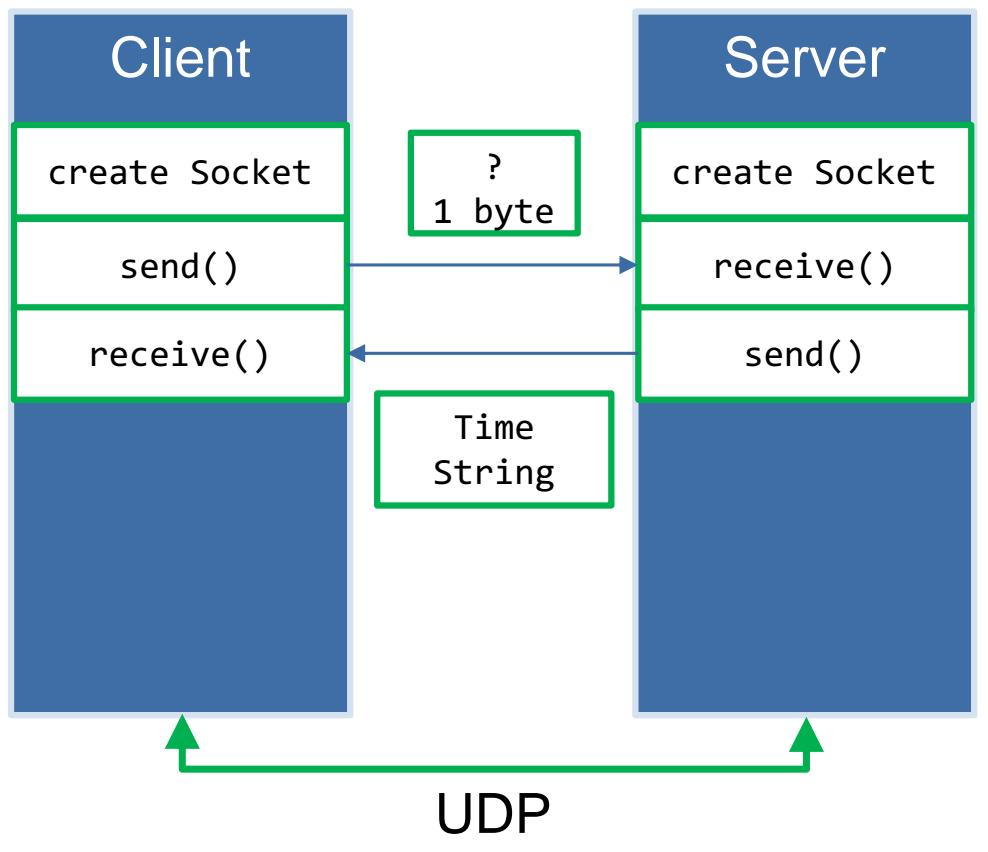
\includegraphics[width=0.5\linewidth]{img/udp_socket}
	\caption{UDP Socket}
	\label{fig:udpsocket}
\end{figure}

\paragraph{Client} \hfill
\begin{lstlisting}
public class DaytimeUDPClient {
	
	private final String targetHost = "localhost";
	private final int targetPort = 5000;
	private final int bufferLength = 256;
	
	public DaytimeUDPClient() throws Exception {
		try (DatagramSocket socket = new DatagramSocket()) {
			// send control datagram
			InetSocketAddress serverAddr = new InetSocketAddress(targetHost, targetPort);
			byte[] controlData = {1};
			DatagramPacket controlPackage = new DatagramPacket(controlData, controlData.length, serverAddr);
			
			socket.send(controlPackage);
			
			// receive answer
			byte[] responseBuffer = new byte[bufferLength];
			DatagramPacket response = new DatagramPacket(responseBuffer, responseBuffer.length);
			socket.receive(response);
			
			System.out.println(new String(responseBuffer, 0, response.getLength()));
		} 
	}
	public static void main(String[] args) throws Exception {
		new DaytimeUDPClient();
	}
}
\end{lstlisting}

\paragraph{Server} \hfill

\begin{lstlisting}
public class DaytimeUDPServer {
	
	private final int targetPort = 5000;
	
	public DaytimeUDPServer() throws Exception {
		
		try (DatagramSocket socket = new DatagramSocket(targetPort)) {
			
			while (true) {
				// control frame
				DatagramPacket packet = new DatagramPacket(new byte[1], 1);
				socket.receive(packet);
				
				// send response
				String dateString = new Date().toString();
				byte[] outBuffer = dateString.getBytes();
				DatagramPacket date = new DatagramPacket(outBuffer, outBuffer.length, packet.getSocketAddress());
				socket.send(date);
			}
		}
	}
	
	public static void main(String[] args) throws Exception {
		new DaytimeUDPServer();
	}
}
\end{lstlisting}




\subsubsection{Berkley Sockets}

Ist ein Message Passing Interface
%TODO: Slide 16 Week 2

\subsubsection{Websockets}

Im Web meistens Server zu Client; aber neu in einigen Fällen synchrone Kommunikation nötig. Websockets werden von vielen Plattformen unterstützt.

\section{Messaging Patterns}

Strukturen, welche zur Datenübertragung genutzt werden:

\subsection{Blocking Receiver Message Pattern}

\begin{figure}[h]
	\centering
	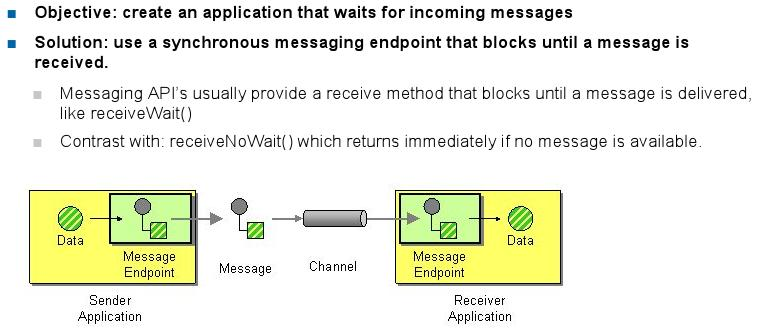
\includegraphics[width=0.7\linewidth]{img/pattern_brmp}
	\caption{Blocking Receiver Message Pattern}
	\label{fig:patternbrmp}
\end{figure}

\subsection{Polling (Non-Blocking) Receiver Message Pattern}

\begin{figure}[h]
	\centering
	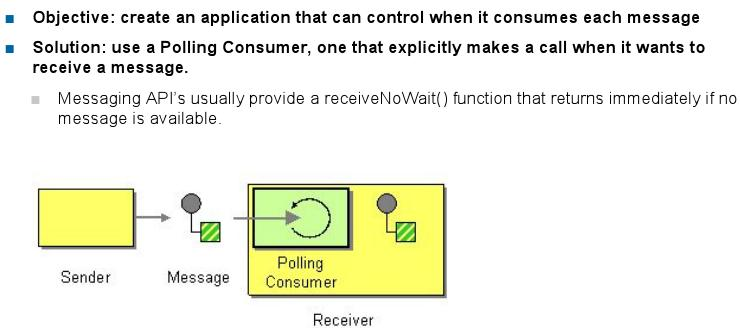
\includegraphics[width=0.7\linewidth]{img/pattern_polling}
	\caption{Polling (Non-Blocking) Receiver Message Pattern}
	\label{fig:patternpolling}
\end{figure}

\newpage

\subsection{Service Activator Message Pattern}

\begin{figure}[h]
	\centering
	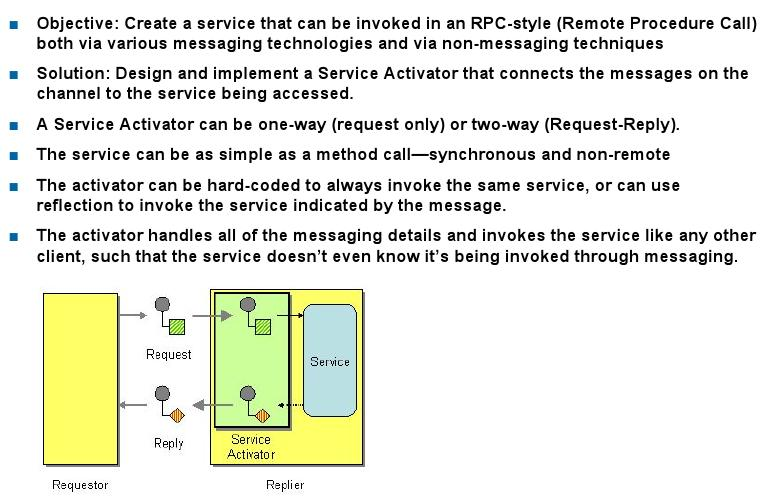
\includegraphics[width=0.7\linewidth]{img/pattern_service_activator}
	\caption{Service Activator Message Pattern}
	\label{fig:patternserviceactivator}
\end{figure}

\subsection{Message Exchange Patterns}

\begin{figure}[h]
	\centering
	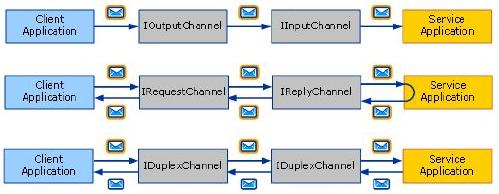
\includegraphics[width=0.7\linewidth]{img/pattern_wcf}
	\caption{Message Exchange Patterns (as defined by WCF)}
	\label{fig:patternwcf}
\end{figure}

\subsubsection{Exchanges and Exchange Types}
Exchanges are AMQP (Advanced Message Queuing Protocol) entities where messages are sent. Exchanges take a message and route it into zero or more queues. There are four types of exchanges:
\begin{description}
	\item[Direct exchange] Delivery based on routing key
	\item[Fanout exchange] Delivery to all the queues that are bound.
	\item[Topic exchange] Route messages to one or many queues based on matching between a message routing key and the pattern that was used to bind a queue to an exchange.
	\item[Headers exchange] Routing on multiple attributes that are more easily expressed as message headers than a routing key
\end{description}

\section{Messaging}
\subsection{Übersicht}
\subsubsection{Merkmale}
Messaging wird heute vielfach als einfacherer Ansatz für die Integration unterschiedlicher Systeme eingesetzt mit den Merkmalen:
\begin{itemize}
	\item Einfachheit
	\item Lose Kopplung
	\item Erweiterbarkeit
	\item Skalierbarkeit
	\item Fehlertoleranz
\end{itemize}

\subsubsection{Queue-basiertes Messaging} Gestattet die flexible und lose Kopplung unterschiedlichster Systeme:

\begin{itemize}
	\item Auf unterschiedlichen Plattformen
	\item In unterschiedlichen Programmiersprachen
	\item Mit völlig unterschiedlichen Message-Formaten (Text, Byte, Objekt)
\end{itemize}

\subsubsection{Enterprise Integration Patterns}
Der Nachrichtenaustausch erfolgt in der Regel mittels eines der zwei Channel-Typen:
\begin{itemize}
	\item Point-to-Point (P2P) liefert jede Nachricht an genau einen Empfänger
	\item Publish-Subscribe kopiert Nachrichten (Lieferung an mehrere Empfänger)
\end{itemize}


\subsubsection{Designentscheide}
Die APIs sind einfach zu benutzen, es müssen aber viele Designentscheidungen getroffen werden:
\begin{itemize}
	\item Message intent (command vs. data)
	\item Returning a response (request-reply)
	\item Huge amounts of data (sequencing)
	\item Slow messages (message expiration)
	\item QoS (guaranteed delivery, transactionality, idempotency)
\end{itemize}

\newpage


\subsection{Message}
A message is a container that consists of:

\begin{figure}[h!]
	\centering
	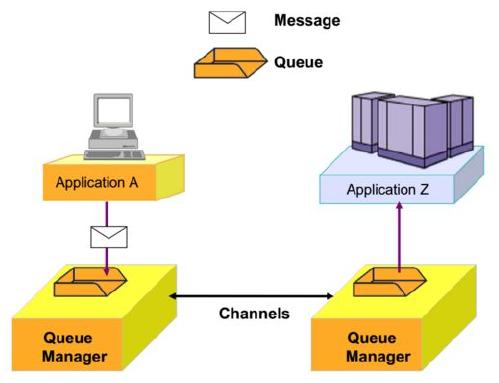
\includegraphics[width=0.5\linewidth]{img/messaging_queue_manager}
	\caption{Messaging Queue manager}
	\label{fig:messagingqueuemanager}
\end{figure}

\begin{description}
	\item[Message Descriptor: ] Identifies the message and contains control information (e.g. message type, and priority) that is assigned to the message by the sending application.
	\item[Message data:] Contains the application data. The structure of the data is defined by the application programs that use it, and the queue manager is largely unconcerned with its format or content.
	\item[Queue Manager] Is responsible for accepting and delivering messages. Maintains queues of all messages that are waiting to be processed or routed. 
\end{description}

\paragraph{Message Queuing Model} \hfill \\
Sender und Empfänger einer Queue können diese entweder aktiv oder passiv abfragen bzw. abfüllen.

\clearpage

\subsection{Two Phase Commit (2PC)}
2PC garantiert, dass alle Teilnehmer ihre Aktion auch wirklich durchführen können. 
\begin{description}
	\item[1. Commit-Request Phase] Koordinator forder alle Teilnehmer auf, die Transaktion probeweise durchzuführen. Die Teilnehmer antworten mit READY oder FAILED.
	\item[2. Commit Phase] Wenn alle Teilnehmer die Transaktion durchführen können (READY) , gibt der Koordinator die Aufforderung die Transaktion wirklich auszuführen. (COMMIT)
\end{description}

\begin{figure}[h]
	\centering
	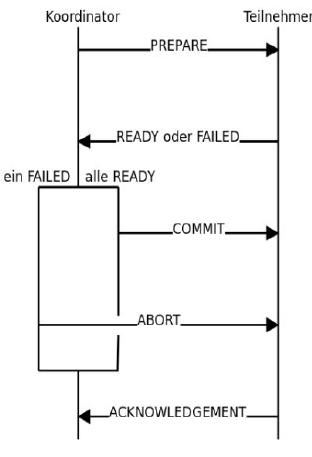
\includegraphics[width=0.3\linewidth]{img/two_phase_commit}
	\caption{Two phase Commit (2PC)}
	\label{fig:twophasecommit}
\end{figure}

\subsection{Java Message Service (JMS)}
Der JMS ist ein Programmierinterface, welches es erlaubt, mit einem Queue Manager zu sprechen.

\subsubsection{Reliability Levels:}
Nachrichten können sowohl persistent als auch nicht-persistent verwaltet werden; es gibt weitere Quality of Service (QoS)-Properties.
\begin{description}
\item[Best effort]	nonpersistent Messages are discarded when a messaging engine stops or fails. Messages might also be discarded if a connection used to send them becomes unavailable or as a result of constrained system resources. \item[Express nonpersistent]	Messages are discarded when a messaging engine stops or fails. Messages might also be discarded if a connection used to send them becomes unavailable.
\item[Reliable nonpersistent]	Messages are discarded when a messaging engine stops or fails.
\item[Reliable persistent]	Messages might be discarded when a messaging engine fails.
\item[Assured persistent]	Messages are not discarded.
\end{description}

\paragraph{Beispiel Sender:} \hfill \\

\begin{lstlisting}[language=java]
Connection connection; connection = connectionFactory.createConnection();
connection.start();
Session session = connection.createSession(mp.transacted, Session.AUTO_ACKNOWLEDGE);
Destination destination = session.createQueue("testQueue");
MessageProducer producer = session.createProducer(destination);
producer.setDeliveryMode(DeliveryMode.PERSISTENT);
TextMessage message = session.createTextMessage("hello");
producer.send(message);
producer.close();
session.close();
connection.close();
\end{lstlisting}

\paragraph{Beispiel Receiver/Consumer:} \hfill \\

\begin{lstlisting}[language=java]
Connection connection = connectionFactory.createConnection();
connection.start();
Session session = connection.createSession(mc.transacted, Session.AUTO_ACKNOWLEDGE);
Destination destination = session.createQueue("testQueue");
MessageConsumer consumer = session.createConsumer(destination);
TextMessage text=(TextMessage) consumer.receive();
consumer.close();
session.close();
connection.close();
\end{lstlisting}

\clearpage


\subsection{Point-to-Point Pattern}

\begin{figure}[h!]
	\centering
	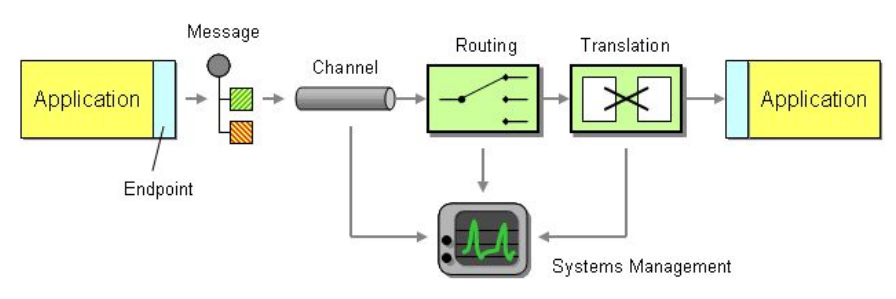
\includegraphics[width=0.7\linewidth]{img/p2p_messaging_pattern}
	\caption{Point-to-Point Messaging Pattern}
	\label{fig:p2pmessagingpattern}
\end{figure}

Beim P2P Pattern wird eine Message in 5 Schritte übertragen:
\begin{description}
	\item[Create] the sender creates the message and populates it with data.
	\item[Send]the sender adds the message to a channel.
	\item[Deliver]the messaging system moves the message from the sender’s 
	computer to the receiver’s computer, making it available to the receiver.
	\item[Receive]the receiver reads the message from the channel.
	\item[Process]the receiver extracts the data from the message
\end{description}

\paragraph{Message Expiration}
Falls der Empfänger nicht verfügbar ist, häuffen sich die Messages in der Queue an. Es empfiehlt sich deshalb, eine Expiration Wert anzugeben, damit die Messages nach einer bestimmten Zeit aus der Queue entfernt werden.

\paragraph{Document Message}
Document Messages werden verwendet um Datenstrukturen auf eine verlässliche Art und Weise zwischen Sender und Empfänger zu übertragen.

\paragraph{Command Message}
Command Messages werden verwendet um Befehle an den Empfänger zu übertragen, die dieser ausführen soll.

\clearpage

\subsection{Publish-Subscribe Pattern}
Beim Publish-Subscribe wird die Message an einen Publish-Subscribe Channel gesendet, welche eine Kopie der Meldung an alle Teilnehmer weiterleitet. (Observer)
\begin{figure}[h!]
	\centering
	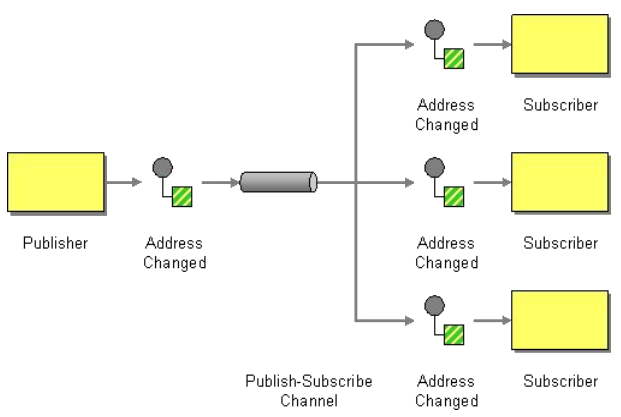
\includegraphics[width=0.7\linewidth]{img/publish_subscribe_messaging_pattern1}
	\caption{Publish Subscribe Integration Pattern}
	\label{fig:publishsubscribemessagingpattern1}
\end{figure}

Man unterscheidet zwischen zwei Typen:
\begin{description}
	\item[Topic-based] Der Publisher beschreibt ein Thema/Typ und der Subscriber interessiert sich für ein oder mehrere Thema/Typen. Die Subscriber erhalten nur noch Meldungen die sich auch interessieren.
	\item[Content-based] Der Subscriber definiert an welchem Inhalt er genau interessiert ist. Es gibt dabei spezifische Attribute an, welche erfüllt sein müssen.
\end{description}


\subsubsection{Publisher JMS}

\begin{lstlisting}[language=java]
public void run() {
	try {
		HelloWorldPublisher mp = new HelloWorldPublisher();
		ActiveMQConnectionFactory connectionFactory = new ActiveMQConnectionFactory(mp.user, mp.password, mp.url);
		Connection connection = connectionFactory.createConnection();
		connection.start();
		Session session = connection.createSession(mp.transacted, Session.AUTO_ACKNOWLEDGE);
		Destination destination = session.createTopic(mp.topicName);
		MessageProducer producer = session.createProducer(destination);
		TextMessage message = session.createTextMessage(mp.messageText);
		producer.send(message);
	} catch (JMSException e) {
	e.printStackTrace();
	} catch (Exception e1) {
	e1.printStackTrace();
	}
}
\end{lstlisting}


\subsubsection{Subscriber JMS}

\begin{lstlisting}[language=java]
public static void main(String[] args) {
	try {
		HelloSubscriber hs = new HelloSubscriber();
		ActiveMQConnectionFactory connectionFactory = new ActiveMQConnectionFactory(hs.user, hs.password, hs.url);
		Connection connection = connectionFactory.createConnection();
		Session session = connection.createSession(hs.transacted, Session.AUTO_ACKNOWLEDGE);
		Destination destination=session.createTopic(hs.topicName);
		MessageConsumer consumer= session.createConsumer(destination);
		connection.start();
		TextMessage text = (TextMessage) consumer.receive();
	} catch (Exception e1) {
		e1.printStackTrace();
	}
}
\end{lstlisting}


\subsection{RabbitMQ}

\begin{figure}[h!]
	\centering
	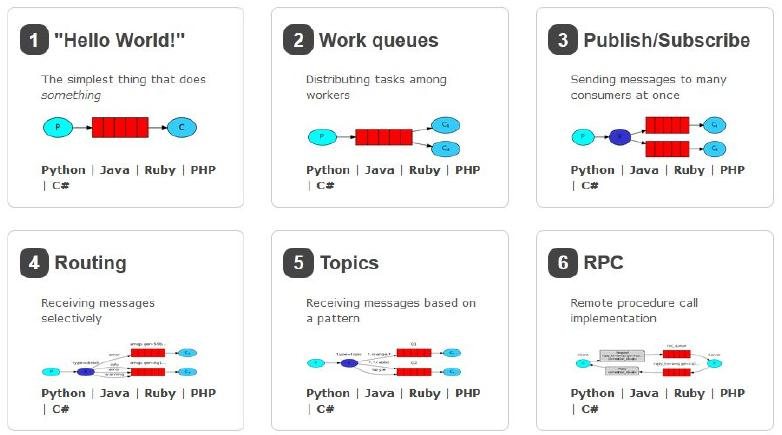
\includegraphics[width=0.8\linewidth]{img/rabbitmq_pattern}
	\caption{RabbitMQ Pattern}
	\label{fig:rabbitmqpattern}
\end{figure}


\section{Remote Procedure Call (RPC)}
Ein Remote Procedure Call verläuft analog zu einem lokalen Funktionsaufruf, jedoch auf einem entfernten Server. Mit RPC lassen sich verteilte, Client-Server Applikationen erstellen.

\begin{itemize}
	\item Der Entwickler muss sich bewusst sein, dass ein RPC wegen Netzwerkprobleme fehlschlagen kann. Der Aufrufer muss mit solchen Fehler umgehen, ohne genau zu wissen, ob die Prozedur beim Server jemals aufgerufen wurde. (Timeout Management)
	\item Nicht idempotente Methoden sind oft keine guten Kanditaten für RPC.
	\item RMI hat eine hohe Kopplung zwischen Client und Server
\end{itemize}

\subsection{Java Remote Method Invocation (RMI)}
\begin{figure}[h]
	\centering
	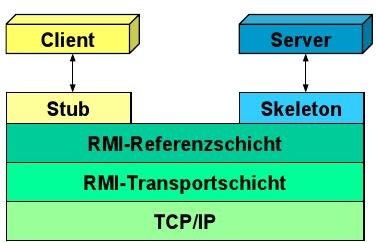
\includegraphics[width=0.5\linewidth]{img/rmi_stack}
	\caption{RMI Stack}
	\label{fig:rmistack}
\end{figure}

\begin{itemize}
	\item Ein Stub ist ein Stellvertreterobjekt (Remote Proxy), das Clientaufruf an Server weiterreicht. Der Procedure Call wird als Message an das OS weitergereicht, welches die Meldung an den Server sendet.
	\item Ein Skeleton nimmt Aufrufe des Stubs entgegen und leitet sie an das Serverobjekt weiter. Solange der Server arbeitet ist der Client typischerweise blockiert. (synchron) Das Serverobjekt (Remote Object) beinhaltet die Methoden, welche aufgerufen werden sollen, sowie einen Status.
	\item Stub und Skeleton implementieren das selbe Interface.
	\item RMI-Referenzschicht stellt Namensdienst (=Registry) zur Verfügung
	\item RMI-Transportschicht verwaltet Verbindungen und wickelt Kommunikation ab
\end{itemize}

\clearpage


\subsubsection{Ablauf}

\begin{figure}[h!]
	\centering
	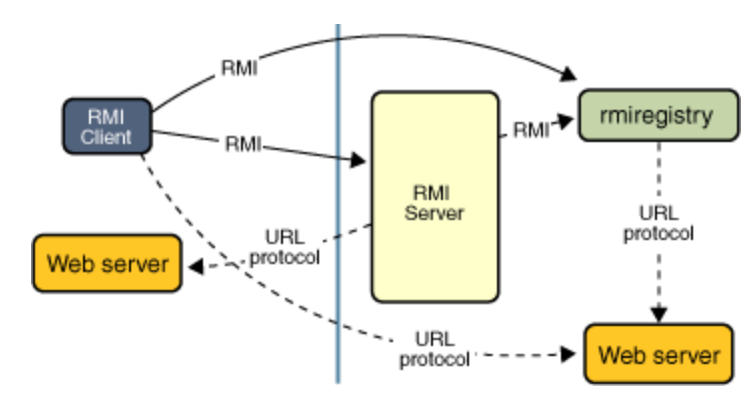
\includegraphics[width=0.7\linewidth]{img/rmi_registry}
	\caption{RMI Registry}
	\label{fig:rmiregistry}
\end{figure}

\begin{enumerate}
	\item Start RMI Registry
	\item Start Server
	\item The server calls the registry to associate (or bind) a name with a remote object.
	\item Start the client
	\item The client looks up the remote object by its name in the server's registry and then invokes a method on it.
	\item The illustration also shows that the RMI system uses an existing web server to load class definitions, from server to client and from client to server, for objects when needed.
	\item Call Methods within remote object
\end{enumerate}


\subsubsection{Implementation}
RMI Klassenimplementationen können vom Server zu den Clients und umgekehrt übertragen werden. Somit können Änderungen an der Businesslogik einmalig beim Server implementiert und an die Clients verteilt werden.

\paragraph{Stub-Klasse in RMI (Remote Proxy)} \hfill \\
Die Stub-Klasse baut Socket-Verbindung zu Server auf (connect-Call). Sie schickt Namen der Methode und Parameter und holt das Ergebnis ab.
\begin{lstlisting}[language=java]
public class HelloImpl_Stub implements Hello {
	Socket socket = new Socket("[hostname]",4711);
	ObjectOutputStream outStream = new ObjectOutputStream(socket.getOutputStream()); 
	// fuer remote Methode sayHello():
	public String sayHello( ) throws RemoteException{
		outStream.writeObject("sayHello"); // simplified example
		ObjectInputStream in = new ObjectInputStream(socket.getInputStream());
		return (String)in.readObject();
	}
}
\end{lstlisting}

\paragraph{Skeleton-Klasse in RMI} \hfill \\
Die Skeleton Klasse erzeugt einen ServerSocket und wartet auf Methoden-Aufrufe von Client und delegiert diesen an das Remote Objekt. Danach liefert sie den Rückgabewert über die Socketverbindung (Port) an den Client zurück.

\begin{lstlisting}[language=java]
public class HelloImpl_Skeleton extends Thread{
	HelloImpl myHello;
	ObjectInputStream inStream = new ObjectInputStream(socket.getInputStream());
	public void run(){
		ServerSocket serverSocket = new ServerSocket(4711);
		Socket socket = serverSocket.accept();
		String method = (String) inStream.readObject(); // simplified ex.
		if(method.equals("sayHello")){
			String return = myHello.sayHello();
			ObjectOutputStream outStream = new ObjectOutputStream(socket.getOutputStream());
			outStream.writeInt(return);
		}
	}
}
\end{lstlisting}

\paragraph{RMI-Programmierung Serverseite} \hfill \\
\begin{lstlisting}[language=java]
// Interface fuer Remote-Methoden (fuer Client und Server)
import java.rmi.Remote;
import java.rmi.RemoteException;
public interface Hello extends Remote {
	String sayHello() throws RemoteException;
}

// Klasse zur Implementierung des Remote-Interface
import java.rmi.RemoteException;
import java.rmi.server.UnicastRemoteObject;
public class HelloImpl extends UnicastRemoteObject implements Hello {
	public HelloImpl() throws RemoteException {
		super();
	}
	public String sayHello() throws RemoteException{
		return "Hello World!";
	}
}

// remote-Objekte erzeugen und in RMI-Registry anmelden
import java.rmi.Naming;
public class HelloServer {
	public static void main(String args[]) {
		try {
			HelloImpl obj = new HelloImpl();
			Naming.rebind("rmi://[hn]/remoteHello", obj);
		}catch (Exception e) { ... }
	}
}
\end{lstlisting}

\subsection{Interface Definition Language (IDL)}

\gls{idl} ist eine plattform-unabhängige Sprache zur Definition von RPC-Interfaces.


\subsection{Web Service Description Language (WSDL)}

\gls{wsdl} ist eine XML-Basierte \gls{idl}, die beim W3C spezifiziert ist. Es ist gut standardisiert (und funktioniert daher auch in mehreren Programmiersprachen), hat allerdings durch XML einen eher grossen Overhead. (4-20x grösser wie der Payload) Man unterscheidet zwischen zwei \gls{wsdl} Styles, wobei der RPC-Style eine festgelegte Struktur hat, der Document-Style dagegen keine Vorgaben definiert. 

\begin{figure}[h]
	\centering
	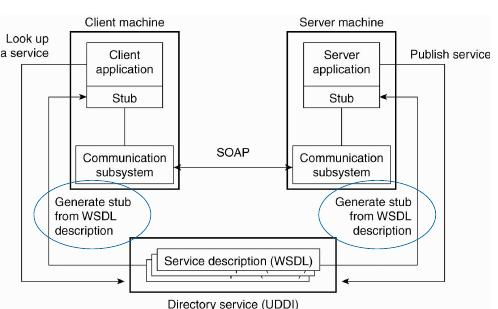
\includegraphics[width=0.7\linewidth]{img/wsdl_overview}
	\caption{\gls{wsdl} Übersicht}
	\label{fig:wsdloverview}
\end{figure}

%TODO: Lecture 10 is missing
\subsection{Flat Nameing}
%TODO
\subsubsection{ARP}
%TODO

\subsection{Structural Nameing}
Hat eine üblicherweise Hierarchie.

%TODO
\subsubsection{DNS}
%TODO?

\begin{description}
	\item[Iterative resolution]	Directly ask all nameservers partially.
	\item[Recursive resolution]	Ask another nameserver to resolve a domain name.
\end{description}

\subsection{Attribute-Based Naming}

Attribute-Based Nameing usually has a Directory Services e.g. LDAP or AD

The main challange is to find a sensible set of attributes (key, value) for all users.

\subsubsection{Bonjour / Zeroconf}

Bonjour / Zeroconf allows automatic name resolving in a local network. It combines DHCP, mDNS (multicast DNS) and SDP (Serice Discovery Protocol). It's aimed at small home networks and only works locally as all parties must be trusted.


\section{Distributed Data Structures}
\subsection{Distributed Hash Tables}

Usually, to Distribute e.g. files over a number $n$ of nodes, one could use a hash function: $location(fileURL) = hashCode(fileURL) \text{ \% } n$. The problem here is that if $n$ changes, the system has to re-distribute all files $>$ the old $n$.

\subsubsection{Chord}

\paragraph{Namespace} Namespache is $2^m$ with typically $m = 128$ or $m = 160$. Nodes are considered to be in a Modulo Ring formation. Each node knows, which node is its successor.

\paragraph{Storing Resources} To store ressources by keys, the storage space is devided up: each node stores keys smaller than its own ID up to the predecessor node.

The $succ(_)$ function is distributed and is used as lookup function. Every host has a $_.successor$ value. If the system is stable, $p.successor = succ(p+1)$.

\begin{description}
	\item[m] m-Bit Identifiers $\rightarrow 2^m$ Namespace size 
	\item[p] ID of a node: p = hash(IP)
	\item[k] Key of a Ressource
	\item[q] Nearest predecessor in finger table
\end{description}

\paragraph{When joining,} the new node lands in a addressspace of a existing node. The predecessors and successors must be convinced that the new node is responsible for its part of the namespace. To allow easy joining, every node also knows his predecessor.

\paragraph{When leaving,} the storage space is transferred to the node's neightbours. The node then leaves the ring.

\paragraph{The finger table} allows faster access ($\mathcal{O}(log \cdot N)$) to more nodes than only the predecessor and successor:

$p.finger[i]$ points to $suc(p + 2^{i-1})$

$p.finger[1] = succ(p + 1) = p.successor$

\paragraph{Lookup} 
\begin{enumerate}
	\item Am I responsible? (is k between me and predecessor) Return my ID to requestor.
	\item Otherwise: Is my successor responsible? Forward request to successor
	\item Otherwise: Forward request clockwisely to predecessor
\end{enumerate}


\section{Synchronization / Logical Clocks}

%TODO, week 12-13


\subsection{Physical Clocks}

%TODO, week 12-13


\subsection{Lamport Logical Clock}

%TODO, week 12-13


\section{Bitcoin}

%TODO, week 14

\appendix

% Code Listings
\lstlistoflistings

% List of figures
\listoffigures

% List of tables
\listoftables

% Bibliography
\bibliographystyle{plain} 
\bibliography{literatur}

\end{document}
